\documentclass[11pt, titlepage]{article}
% Common packages/environments to remove clutter

% Packages
\usepackage[utf8]{inputenc}
\usepackage{amsmath, amsfonts, amssymb, amsthm, enumitem, tikz, import, mathtools}
\usepackage[
  top=2cm,
  bottom=2cm,
  left=3cm,
  right=3cm,
  headheight=17pt,
  includehead, includefoot,
  heightrounded,
]{geometry}

% Problem environment
\newtheoremstyle{emptyplain}
    {}          % default space above
    {}          % default space below
    {}          % default body font
    {}          % no indent
    {\bfseries} % head font
    {.}         % punctuation after theorem head
    { }         % space after theorem head
    {#3}
\theoremstyle{emptyplain}
\newtheorem*{problem}{}

% Solution Environment
\newenvironment{solution}{
  \begin{proof}[Solution]
    \vspace{-2px}
    \setlength{\parskip}{4px}
    \setlength{\parindent}{0px}
}{
\end{proof}
}


% Opening
\title{Math 2552 Written HW Set 8}
\author{Akash Narayanan}
\date{March 30, 2021}

\begin{document}
    \maketitle

    % Judson 5.1 #3
    \begin{problem}[Judson 5.1.3]
        For the below system,
        \begin{enumerate}[label=\alph*.]
            \item Plot and label the nullclines for equation in the system.
            \item Find all of the equilibrium solutions for the system.
            \item Use the Jacobian to classify each equilibrium solution (spiral
                source, nodal sink, etc.).
        \end{enumerate}
        \begin{align*}
            \frac{dx}{dt} &= x(5-x-y) \\
            \frac{dy}{dt} &= y(20-x-2y)
        \end{align*}
    \end{problem}

    \begin{solution}
        We plot the slope field and the nullclines for the system of
        differential equations. The nullclines are found by setting each
        equation in the system equal to zero, yielding the four equations
        \begin{align*}
            x &= 0 & y &= 0 \\
            5 - x - y &= 0 & 20 - x - 2y &= 0
        \end{align*}
        and the following graph. Red lines are $x$-nullclines and green lines
        are $y$-nullclines.
        \begin{center}
            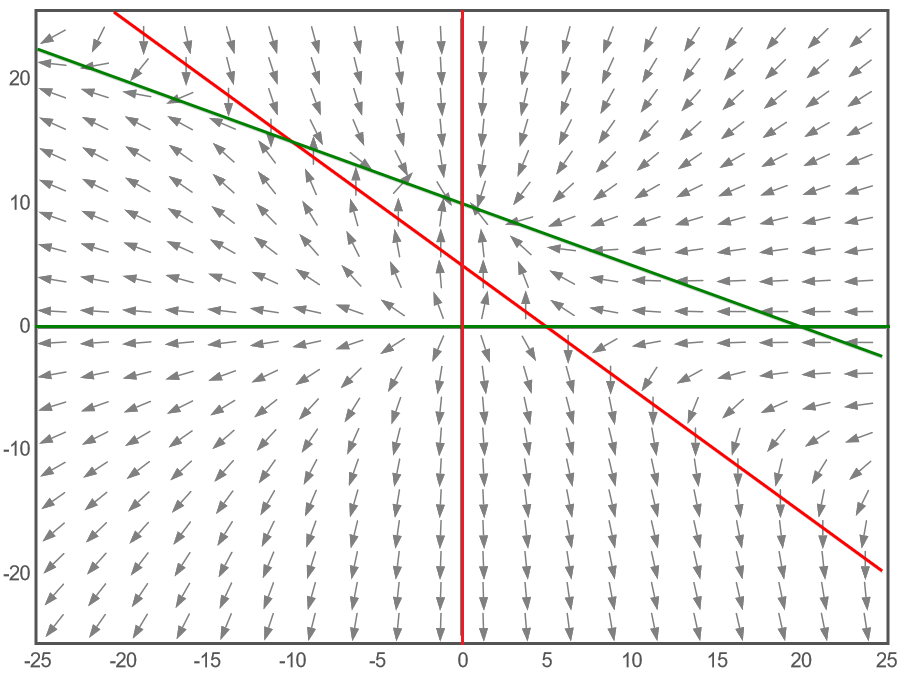
\includegraphics[scale=0.5]{media/slopeField1.png}
        \end{center}
        Equilibrium solutions are where both derivatives are zero, or where
        different nullclines intersect. Easily seen are the points $(0, 0), (0,
        10),$ and $(5, 0)$. The last point is found by setting $5 - x - y = 20
        - x - 2y$, or $y = 15$, yielding the point $(-10, 15)$.

        To classify each solution, we start by calculating the Jacobian,
        \[
        J = 
        \begin{pmatrix}
            \frac{\partial x'}{\partial x} & \frac{\partial x'}{\partial y}
            \\[1ex]
            \frac{\partial y'}{\partial x} & \frac{\partial y'}{\partial y}
        \end{pmatrix} = 
        \begin{pmatrix}
            -2x-y+5 & -x \\
            -y & -4y-x+20
        \end{pmatrix}
        \] 
        Evaluating the Jacobian at each critical point allows us to classify
        them. We begin with $(0, 0)$:
        \[
            J(0, 0) = 
            \begin{pmatrix}
                5 & 0 \\
                0 & 20
            \end{pmatrix}
        \] 
        By inspection, the matrix has eigenvalues 5 and 20. Since both
        eigenvalues are positive and real, the point is a nodal source.
        Next, we have
        \[
            J(0, 10) = 
            \begin{pmatrix}
                -5 & 0 \\
                -10 & -20
            \end{pmatrix}
        \] 
        Again by inspection, the matrix has eigenvalues -5 and -20. Both
        eigenvalues are negative and real so the point is a nodal sink.
        Evaluating the third point, we find
        \[
            J(5, 0) = 
            \begin{pmatrix}
                -5 & -5 \\
                0 & 15
            \end{pmatrix}
        \] 
        By inspection, the matrix has eigenvalues -5 and 15. Both eigenvalues
        are real but differ in sign so the point is a saddle.
        Finally, we find
        \[
            J(-10, 15) = 
            \begin{pmatrix}
                10 & 10 \\
                -15 & -30
            \end{pmatrix}
        \] 
        The characteristic polynomial of this matrix is $\lambda^2 + 20\lambda -
        150$ and the eigenvalues are $-10 \pm 5 \sqrt{10}$. Both eigenvalues are
        real but differ in sign so the point is a saddle.
    \end{solution}

    \pagebreak

    % Judson 5.1 #5
    \begin{problem}[Judson 5.1.5]
        For the below system,
        \begin{enumerate}[label=\alph*.]
            \item Plot and label the nullclines for equation in the system.
            \item Find all of the equilibrium solutions for the system.
            \item Use the Jacobian to classify each equilibrium solution (spiral
                source, nodal sink, etc.).
        \end{enumerate}
        \begin{align*}
            \frac{dx}{dt} &= x(y^2-x) \\
            \frac{dy}{dt} &= y(y-1)
        \end{align*}
    \end{problem}

    \begin{solution}
        As above, we plot the slope field and nullclines for the system with the
        same colorscheme. Setting the derivatives in the system equal to zero
        yields the equations
        \begin{align*}
            x &= 0 & y &= 0 \\
            x &= y^2 & y &= 1
        \end{align*}
        and the following graph where red lines are $x$-nullclines and green
        lines are $y$-nullclines.
        \begin{center}
            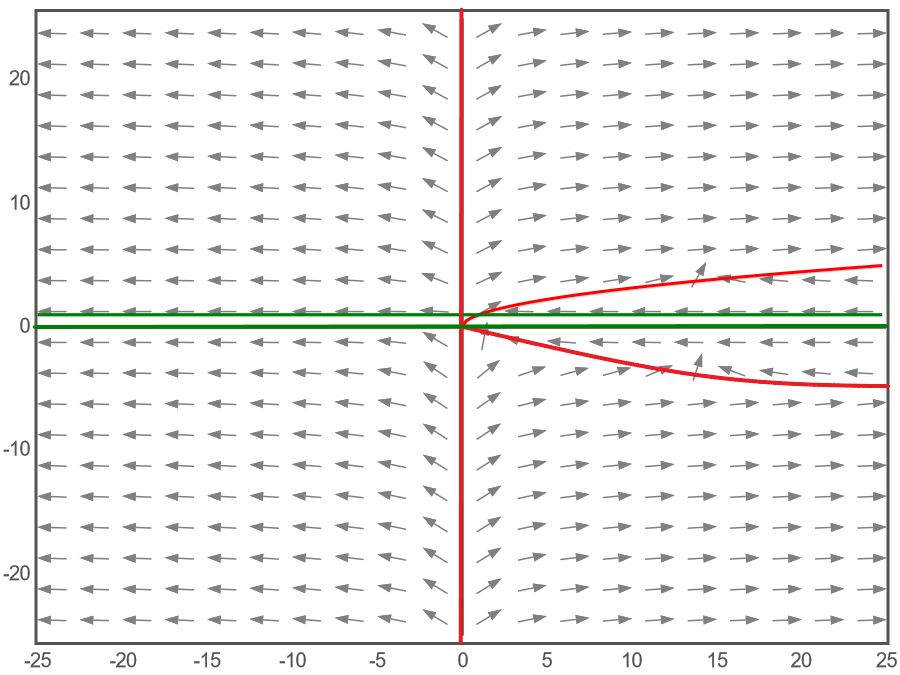
\includegraphics[scale=0.3]{media/slopeField2.png}
        \end{center}
        We find the equilibrium points by calculating where equilibrium points
        intersect. Letting $x = 0$ yields the points $(0, 0)$ and $(0, 1)$. The
        third point is found by letting $y = 1$ and seeing that $x = 1$, meaning
        the third point is $(1, 1)$.

        Next, we calculate the Jacobian.
        \[
        J = 
        \begin{pmatrix}
            \frac{\partial x'}{\partial x} & \frac{\partial x'}{\partial y}
            \\[1ex]
            \frac{\partial y'}{\partial x} & \frac{\partial y'}{\partial y}
        \end{pmatrix} =
        \begin{pmatrix}
            y^2 - 2x & 2xy \\
            0 & 2y-1
        \end{pmatrix}
        \] 
        Evaluating at the equilibrium points, we find
        \[
            J(0, 0) = 
            \begin{pmatrix}
                0 & 0 \\
                0 & -1
            \end{pmatrix}
        \] 
        which, by inspection, has eigenvalues 0 and -1. Since one eigenvalue is
        negative and the other is zero, the critical point is a semi-stable node.
        The second equilibrium point yields
        \[
            J(0, 1) = 
            \begin{pmatrix}
                1 & 0 \\
                0 & 1
            \end{pmatrix}
        \] 
        which has eigenvalue 1. Thus, the critical point is a nodal source.
        Finally, the last equilibrium point gives
        \[
            J(1, 1) =
            \begin{pmatrix}
                -1 & 2 \\
                0 & 1
            \end{pmatrix}
        \] 
        By inspection, this matrix has eigenvalues -1 and 1. Since they are both
        real and differ in sign, the critical point is a saddle.
    \end{solution}

    \pagebreak

    % Trench 6.2 #5
    \begin{problem}[Trench 6.2.5]
        A 16 lb weight stretches a spring 6 inches in equilibrium. It is
        attached to  a damping mechanism with constant $c$. Find all values of
        $c$ such that the free vibration of the weight has infinitely many
        oscillations.
    \end{problem}

    \begin{solution}
        Converting 16 lb to mass yields $16 / 32 = 0.5$ slugs. Furthermore, we
        have $k = 16 / 0.5 = 32$ lb/ft. so the equation of motion for the
        problem is
        \[
        0.5y'' + cy' + 32y = 0.
        \] 
        The free vibration has infinitely many oscillations if and only if the
        motion is underdamped, or $c < \sqrt{4mk}$. The characteristic equation
        of the differential equation is
        \[
        0.5r^2 + cr + 32 = 0
        \] 
        and it has roots
        \[
        r = -c \pm \sqrt{c^2 - 64}
        \] 
        The motion is underdamped if $c < \sqrt{64} = 8$. Thus, the set of
        values of $c$ such that the free vibration of the weight has infinitely
        many oscillations is the interval $0 \leq c < 8$.
    \end{solution}
\end{document}
